
\documentclass[a4paper,12pt]{article}
\usepackage[czech]{babel}
\usepackage[pdftex]{graphicx}
\usepackage[utf8]{inputenc}
\usepackage{amsthm}
\usepackage{amsfonts}
\usepackage{wrapfig}
\usepackage{verbatim} 
\usepackage[unicode]{hyperref}

\setlength{\hoffset}{-1.3cm} % 1.7
\setlength{\voffset}{-2cm} % 2
\setlength{\textheight}{23.3cm}
\setlength{\textwidth}{16.4cm}


\usepackage[font=small,labelfont=bf,tableposition=top]{caption}
\DeclareCaptionLabelFormat{andtable}{#1~#2  \&  \tablename~\thetable}

\newcommand{\HRule}{\rule{\linewidth}{0.2mm}}

\newtheorem{define}{Definice}

\begin{document}

% Uvodni strana

\begin{titlepage}

\begin{center}


FIT VUT v Brně, 2012\\[1.5cm]

\includegraphics[width=7cm]{./img/fit-cz.png}\\[1cm]

% Title
\HRule \\[0.4cm]
{\huge \bfseries Swarm Intelligence}\\[0.1cm]
{\LARGE Inteligence roje}
\HRule \\[0.8cm]

{\large Učební text k předmětu Inteligentní systémy (SIN)}\\[1cm]

\vfill

\end{center}

\begin{minipage}{0.4\textwidth}
\begin{flushleft} \large
\emph{Autoři textu:}\\
Bc. Tomáš \textsc{Kimer}\\
Bc. Stanislav \textsc{Heller}
\end{flushleft}
\end{minipage}

\end{titlepage}


% Obsah
\tableofcontents
\newpage

% -----------------------------------------------------------------------------
% UVOD
% -----------------------------------------------------------------------------

\section{Úvod}
Inteligence roje ({\it angl. Swarm Intelligence}) je jedním z relativně nových
paradigmat\footnote{Jako první tento pojem představil G.Beni v roce 1989, viz
\cite{BeniWang89}.} v~oblasti umělé inteligence. Již dlouhou dobu před prvním
využitím inteligence roje v informatice byli biologové fascinováni způsoby,
jakými dokáže hmyz řešit problémy, které jsou nad síly jedince a přesností
a efektivitou, s jakou skupina jedinců komunikuje a interaguje; mravenci dokáží
společnými silami přemístit relativně velké objekty, hejno ptáků letí synchronně, 
včely při hledání místa, na kterém založí nové hnízdo, využívají sofistikovaného
způsobu vysílání průzkumníků. Tyto a další příklady inteligentního chování hmyzu
v přírodě vedly výzkumníky k myšlence využití těchto vlastností ve výpočetní
technice, zvláště v oboru umělé inteligence.

Při pohledu na swarm jako inteligentní systém, jej lze definovat jako skupinu
{\it N} agentů, kteří společně kooperují a interagují, aby dosáhli nějakého cíle.
Význam označení agent zde nemá stejný význam jako v~{\it multiagentních systémech};
většina rojů je složena z {\it jedinců}, kteří nejsou příliš inteligentní, mají omezené
schopnosti a samostatně nevykazují žádné známky inteligence. Systém obsahující větší
množství takových agentů ale při vhodném nastavení může řešit i poměrně složité
problémy. Příkladem takových problémů může být optimalizace (obecně {\it NP} problémy),
kooperativní transport v~oblasti robotiky či problémy, u kterých je třeba vyvinout
řešení s~vysokou adaptabilitou a schopností samoopravy. Největší zájem o tuto poměrně
novou disciplínu je v oborech, které souvisí vojenstvím, telekomunikacemi a v~medicíně.

Pro další výklad je třeba definovat některé často užívané pojmy. Je třeba upozornit,
že přesné matematické definice těchto jevů v~oblasti aplikace v informatice v~současnosti
neexistují. Bohužel, mezi akademiky neexistuje shoda v oblasti významu následujících pojmů
a proto tyto definice uvádíme spíše pro ilustraci.
\begin{define}
  {\bf Emergentní jev} představuje vznik netriviálních globálních vlastností systému na
  základě množství jednoduchých lokálních interakcí. Tyto vlastnosti nelze odvodit studiem
  jednotlivých entit nezávisle na ostatních složkách systému.
\end{define}

\begin{define}
  {\bf Samoorganizace} je vlastnost systému, který je autonomní, adaptivní a jeho 
  části vykazují emergentní chování. \cite{Wuchner07}
\end{define}
Původ tohoto termínu sahá do 50. let 20. století, kdy spadal do oblasti obecné teorie
systémů a kybernetiky. Často jsou v souvislosti se samoorganizací zmiňovány pojmy
{\it pozitivní a negativní zpětná vazba}, které jsou základem většiny samoorganizujících
se systémů.

\begin{define}
  {\bf Stigmergie} je mechanismus komunikace, kde si jedinci nepředávají informace přímo,
  ale pouze nepřímo přes prostředí. \cite[s.6]{Heylighen99}
\end{define}
Původ slova pramení v řečtině ze spojení slov "stigma" (znak) a "ergon" (práce). Příkladem
stigmergické komunikace je spolupráce mravenců, kteří na zemi zanechávají feromonové stopy
na cestě za potravou a předávají si tak informaci o tom, kde lze její zdroj nalézt.

\begin{define}
  {\bf Kolektivní inteligence} je schopnost skupiny jedinců řešit problém lépe nebo kvalitněji,
  než by jej řešil jednotlivec. \cite[s.1]{Heylighen99}
\end{define}


\subsection{Biologický základ inteligence roje} \label{sub:biolzakl}
Hmyzu, který se shlukuje do větších seskupení, interaguje s ostatními členy skupiny,
říkáme {\it společenský hmyz}. Ve většině případů, které jsou v přírodě pozorovány,
takový hmyz vykazuje při řešení základních problémů poměrně vysokou inteligenci. Mezi
tento hmyz řadíme např. mravence, včely, vosy, kobylky, termity a další. V této
kapitole se budeme věnovat popisu některých jevů, se kterými se ve spojitosti s~chováním
společenského hmyzu můžeme setkat. Tento popis\footnote{Pokud není uvedeno jinak, veškerý
materiál k~textu této kapitoly je čerpán z \cite{Beekman08SwarmBio}.} bude uveden v~míře
nezbytné pro pochopení problematiky, avšak se zřetelem na technické, nikoli biologické
zaměření tohoto učebního textu.

\paragraph{Mravenci: hledání potravy.}
Při vyhledávání potravy mravenci využívají stigmergický přístup ke komunikaci. Pokud mravenec
nalezne zdroj potravy, na cestě zpět zanechává na zemi substanci, která je nazývána {\it feromon}.
Ostatní mravenci cítí přítomnost feromonů a mají tendenci sledovat cestu, na které je koncentrace
feromonů vyšší \cite{Dorigo06antcolony}. Pokud po jedné cestě projde více mravenců, tím více po
sobě zanechají feromonů a tím spíše po této trase půjde větší počet mravenců v budoucnosti.

Feromonová stopa ale po čase mizí; tomuto procesu říkáme {\it vypařování}. Tímto mechanismem se
mravenci dokáží velmi rychle a efektivně přizpůsobovat změnám podmínek - např. pokud zdroj
potravy zmizel či pokud na cestě za potravou vznikla překážka.

\paragraph{Mravenci: přesun kořisti.}
Dalším ze známých jevů u mravenců je kooperativní transport. Pokud mravenci uloví kořist, která
je velká a příliš těžká pro jednotlivce, aby ji odtáhl, více mravenců spojí síly a společně
kořist odnesou.

\paragraph{Mravenci: výběr místa pro mraveniště.}
Chování mravenců\footnote{Toto chování se vztahuje ke druhu {\it Temnothorax albipennis}.} při
průzkumu a hledání místa pro nové mraveniště se liší od způsobu hledání potravy. Nevyužívají
feromonové stopy, ale dvou jiných způsobů: párování ({\it tandem running}) a přenosu ({\it social
carrying}). Průzkumníci, kteří nalezli vhodné místo pro nové mraveniště, si vyberou druhého
mravence do páru a toho dovedou na nalezené místo (párování). Tím jej naučí, jak se má k~místu
dostat a pokud takto zaučený mravenec usoudí, že se jedná o dobré místo, začne tam provázet
další mravence. Výsledkem tohoto procesu je několik míst, na kterých se soustředí velké množství
mravenců, protože méně kvalitní lokality nebudou mravence tolik lákat. Aby bylo zajištěno,
že bude vybráno pouze jedno místo, od určitého počtu jedinců na vybraném místě se mravenci
přestanou párovat (ve smyslu prohledávání) a jedinci na starém místě (včetně larev, vajíček atp.)
jsou přeneseni na místo nové. Tím je zajištěno, že proces výběru konverguje.

\paragraph{Včely: plnění pláství.}
Prakticky přesné šestiúhelníkové buňky nejsou jedinou zajímavostí včelích pláství. Při plnění
pláství nektarem, vajíčky a pylem včely dodržují zvláštní vzor, který vytváří tři oddělené
regiony: ve vnitřním kruhu jsou nakladena vajíčka, ze kterých se vylíhnou nové včely, okolo
této oblasti je vytvořen pruh buněk, které obsahují pyl, který je určen jako potrava pro larvy.
Na vnějším okraji plástve je pak oblast, ve které se vyskytuje nektar, který je pak přetvořen
na med. Celý vzor je znázorněn na obrázku \ref{fig-honeycomb}.

Umístění pylu blízko larev je velmi efektivní - snižuje čas a námahu pro krmení. Tvorba
tohoto vzoru ale není náhodná. Královna si buňky, do kterých naklade vajíčka, vybírá tak, aby
byly dostatečně vzdálené od kraje plástve a preferuje místa, kde se vajíčka již v okolí vyskytují.
Při krmení včely vybírají vždy buňky, které jsou nejblíže larvám. I v~případě, že by byl pyl
a nektar nakladen náhodně, vznikne na plástvi díky vybírání nejbližších buněk vždy podobný
(výše popsaný) vzor, což bylo dokázáno simulací (Camazine 1991). Tento princip je další ukázkou
emergentního jevu, kdy výskyt vzoru na úrovni plástve je tvořen lokálními interakcemi na úrovni
buněk.

\begin{figure}[here]
  \centering
  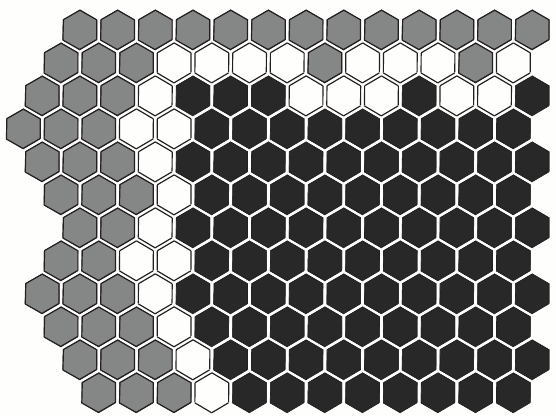
\includegraphics[width=10cm]{./img/comb.png}
  \caption{Typický vzor rozmístění medu (šedý), pylu (bílý) a vajíček (černé) na výřezu
   včelí plástve v horním levém rohu. Převzato z \cite{Beekman08SwarmBio}.}
  \label{fig-honeycomb}
\end{figure}


\paragraph{Včely: hledání nového místa pro hnízdo.}
Včely při vyhledávání místa pro hnízdo využívají systému průzkumu a zpětné vazby. Průzkumníci
se vydávají hledat nové místo do všech směrů od současného hnízda. V případě, že průzkumník
našel nové místo pro hnízdo, při návratu zpět do hnízda provádí jistý druh "tance". Kvalita
místa je v~tanci projevena jeho délkou a pohyby, které včela provádí. Na jejich základě dává
roji vědět, jak daleko leží nalezené místo a jakou kvalitu má. Na počátku procesu vyhledávání
se mnoho průzkumných včel vrací do roje a podávají zprávu o místech, které našly. Po několika
hodinách proces konverguje a pro některá místa již žádné včely netančí; těsně před tím, než se
roj vydá na cestu, většina průzkumných včel tančí tanec reprezentující jedno místo, na které
roj poletí.

\paragraph{Včely: přesun roje.}
Přesun skupiny hmyzu může být považován za jeden ze stěžejních problémů, který hmyz musí
řešit při změně místa hnízda. Existují dva extrémní případy jak se skupina "rozhoduje", kterým
směrem se bude pohybovat\cite{Blum08SwarmInt}:
\begin{itemize}
  \item buď se skupina "dohodne", tedy každý člen zná přibližný směr pohybu
  \item nebo existuje poměrně malé množství informovaných členů (tzv. {\it vůdců}), kteří
        neinformovanou většinu vedou.
\end{itemize}
V druhém případě je třeba, aby {\it vůdci} dokázali skupinu nějakým mechanismem ovládat. V principu
lze v přírodě pozorovat, že neinformovaní členové vždy přizpůsobují směr svého pohybu ostatním.
Toho vůdci využívají a díky své tendenci letět správným směrem mají vliv na směr pohybu skupiny.
Další možností je, že vůdci vysílají určitý druh signálů, kterým skupinu řídí.

Ve včelím roji ví o novém směru pohybu pouze asi 5\% členů, jedná se tedy o princip neinformované
většiny a informovaných vůdců.


\subsection{Otázky}
\begin{enumerate}
  \item Jak se liší přístup inteligence roje od klasických multiagentních systémů?
  \item Jaké problémy jsou řešitelné pomocí inteligence roje?
  \item Vysvětlete pojmy emergence, samoorganizace a kolektivní chování.
  \item Popište způsob, jakým si mravenci předávají informace při vyhledávání potravy.
\end{enumerate}

\newpage


% -----------------------------------------------------------------------------
% OPTIMALIZACE (ACO, PSO, GWO atp.)
% -----------------------------------------------------------------------------

\section{Inteligence roje v optimalizaci}
%Obecné kecy o optimalizaci...
Inteligence roje má v optimalizaci jedno z nejdůležitějších využití. Optimalizací rozumíme řešení
nějakého {\it optimalizačního problému}, který se skládá z hledání optima (maxima či minima)
nějaké účelové funkce. Mnoho teoretických úloh i úloh z reálného světa vede právě na řešení úlohy
optimalizace. Jako reálné příklady můžeme uvést plánování odjezdů vlaků ({\it train scheduling}),
vytváření rozvrhů ({\it timetabling}), optimalizaci tvarů ({\it shape optimization}), návrh
telekomunikačních sítí či problémy z výpočetní biologie ({\it computational biology}). Mnoho
těchto problému bylo zobecněno na nějaký známý, {\it NP-těžký} problém, jako je například {\it problém
obchodního cestujícího} (TSP), což je jeden z nejznámějších {\it NP-těžkých} problémů kombinatorické
optimalizace \cite{Blum08SwarmOpt}.

%\medskip
\subsection{Úvod}

Obecně můžeme optimalizační problém $\mathcal{P}$ definovat jako trojici $(S,\omega,f)$, kde $S$
je prohledávací prostor definovaný na konečné množině proměnných $X_i,i=1,\dots,n$ (přípustná
množina), $\omega$ je množina omezujících podmínek nad těmito proměnnými a
$f:S\rightarrow\mathbb{R}^{+}$ je účelová funkce, která přiřazuje ohodnocení každému prvku (neboli
řešení) z $S$. Pokud mají proměnné diskrétní doménu (definiční obor), hovoříme o diskrétní
(kombinatorické) optimalizaci, v opačném případě hovoříme o optimalizaci spojité (existuje i
kombinovaná).

Cílem optimalizace je najít řešení $s\in S$ optimalizačního problému $\mathcal{P}$ takové, že
$f(s)\leq f(s^{\prime}),\forall s^{\prime}\in S$ (v případě, že chceme účelovou funkci
minimalizovat), či $f(s)\geq f(s^{\prime}),\forall s^{\prime}\in S$ (v případě, že ji chceme
maximalizovat). V reálných problémech se často můžeme setkat s optimalizací několika účelových
funkcí zároveň ({\it víceúčelová optimalizace}), hledání více než jednoho optima účelové funkce
({\it multimodální optimalizace}), či optimalizací {\it dynamickou} (schopnost adaptace na změnu
optima v čase) \cite{Blum08SwarmOpt}.

\subsubsection{Metody optimalizace}
%\medskip

Vzhledem k praktické důležitosti optimalizačních problémů bylo na jejich řešení vyvinuto mnoho
algoritmů. V kontextu kombinatorické optimalizace můžeme tyto algoritmy klasifikovat na úplné a
aproximační. Úplné algoritmy zaručeně najdou pro každý, konečně velký, kombinatorický problém
optimální řešení v omezeném čase. Pro problémy, které jsou {\it NP-těžké}, ale neexistuje žádný
algoritmus, který najde řešení v polynomiálním čase ($P\neq NP$). Úplný algoritmus by v nejhorším
případě potřeboval exponenciální výpočetní čas, což by, vzhledem k praktickému využití, vedlo k
velmi dlouhým výpočetním časům. Proto je stále vetší pozornost věnována metodám aproximačním, kam
lze zařadit i algoritmy inspirované inteligencí roje. Sice u nich nemáme jistotu nalezení
optimálního řešení, na druhou stranu ale nalezneme řešení alespoň blízké optimálnímu, a to ve
významně zkráceném čase (prohledávací prostor není obvykle prohledán celý) \cite{Blum08SwarmOpt}.

Aproximační metody můžeme rozdělit na {\it lokální prohledávání} (iterativní zlepšování počátečního
řešení až do uváznutí v lokálním extrému) a {\it konstruktivní algoritmy} (budování řešení s využitím
heuristické znalosti). Metody inteligence roje jsou rozšířením tradičních konstruktivních heuristik o
schopnost využití zkušeností získaných v průběhu řešení daného problému (tzv. {\it metaheuristiky}).
Zde můžeme zařadit například i evoluční algoritmy. %TODO upravit
%heuristiky vs metaheuristiky
%TODO jeste neco o spojite? nebo napsat ze ji tu neresime?

\subsubsection{Přínos inteligence roje v optimalizaci}

Významným přínosem technik inteligence roje je oproti jiným metodám obvykle vetší rychlost, nízká
výpočetní náročnost a schopnost poskytnout alespoň přibližné řešení tam, kde nám často ani není známo,
zda existuje nějaký exaktní postup, jak řešení najít. %TODO rozvest, overit

%\medskip

Dvě nejvýznamnější techniky pro získání přibližných řešení v rozumném čase jsou optimalizace mravenčí
kolonií ({\it ant colony optimization}) a optimalizace hejnem částic ({\it particle swarm optimization}).


\subsection{Optimalizace mravenčí kolonií (ACO)}
%Pro algoritmy typu ACO bude vhodné využít \cite{Dorigo06antcolony}.
Optimalizace mravenčí kolonií byla jedna z prvních technik aproximační optimalizace inspirovaná
inteligencí roje (konkrétně hledáním potravy u mravenců, viz \ref{sub:biolzakl}).

\subsubsection{Vznik metody}
\dots

\subsubsection{Princip}
\dots

\subsubsection{Aplikace na TSP}
\dots

\subsubsection{Další využití}



%TODO Srovnání s genetickými algoritmy?

\subsection{Optimalizace hejnem částic (PSO)}
%Tady se bude brát hlavně z \cite{Blum08SwarmOpt}.
Optimalizace hejnem částic je populačně založená stochastická optimalizační metoda inspirovaná
shlukováním zvířat či hmyzu (například hejna ptáků či ryb). PSO optimalizuje problém\dots


\subsubsection{Vznik metody}
\dots

\subsubsection{Princip}
\dots

\subsubsection{Využití}
Optimalizace algoritmy PSO má široké využití -- od klasických problémů, jako je plánování, TSP,
trénování neuronových sítí či {\it assignment problem}, až po vysoce
specializované aplikace, jako je {\it reactive power} a {\it voltage control}, {\it biomedical image registration},
či dokonce skládání hudby. V posledních letech byly metody PSO taky oblíbené ve víceúčelové a dynamické optimalizaci.
%TODO metody cesky (jak prelozit? co jsou zac?)

Jednou z prvních aplikací metod PSO byl vývoj metod učení neuronových sítí. PSO bylo využito jako náhrada
tradičního {\it back-propagation} algoritmu pro učení vícevrstvého perceptronu. Díky rychlé konvergenci může
užití PSO v trénování neuronových sítí ušetřit značný výpočetní čas ve srovnání s jinými
optimalizačními metodami.


%\subsection{Stochastic diffusion search (SDS)}
%\url{http://en.wikipedia.org/wiki/Stochastic_diffusion_search}
%Další zdroje?

\subsection{Další metody}
Následuje seznam některých dalších metod se stručným popisem. Seznam nelze brát jako úplný, jelikož se toto, relativně mladé, odvětví stále vyvíjí a neustále vzniká mnoho modifikací původních algoritmů, hybridní metody či
přístupy zcela nové.

\begin{description} %TODO jine formatovani? - subsubsection?, paragraph?

\item[Optimalizace včelím rojem (BCO)] zahrnuje celou skupinu algoritmů, které se inspirují chováním včel.
Zásadní roli zde hraje přímá výměna informace mezi jednotlivými včelami na rozdíl od užití feromonu mravenčí
kolonií. Obvykle je roj rozdělen na specializované skupiny: královny, průzkumné včely vyhledávající nové zdroje
potravy, včely následující úspěšné průzkumné včely a podobně. ({\bf z wiki - upravit})

\item[Optimalizace hejnem světlušek (GSO)] je metoda, ve které její autoři vybavují  každého člena hejna
virtuální svítivou látkou (luciferin) v závislosti na jeho úspěšnosti při procházení prohledávacím prostorem.
Čím úspěšnější, tím více září a přitahuje ke své pozici ostatní světlušky. U každé světlušky se zároveň
předpokládá omezená vzdálenost, kam až dohlédne. Tato vzdálenost se i dynamicky vyvíjí a algoritmus dosahuje
zajímavých výsledků při multimodální optimalizaci. ({\bf z wiki - upravit})

\item[Stochastic diffusion search (SDS)] je metoda, která oproti ACO využívá přímou ({\it one-to-one}) komunikaci
mezi agenty (inspirovanou jedním druhem mravenců). {\it Agents perform cheap, partial evaluations of a hypothesis (a candidate solution to the search problem). They then share information about hypotheses (diffusion of information) through direct one-to-one communication. As a result of the diffusion mechanism, high-quality solutions can be identified from clusters of agents with the same hypothesis. The operation of SDS is most easily understood by means of a simple analogy – The Restaurant Game.} ({\bf z wiki - prelozit, upravit, popis hry?})

\item[Co vybrat dál?] A kolik \dots ? \url{http://en.wikipedia.org/wiki/Swarm_intelligence}

\end{description}


\subsection{Otázky}
\begin{enumerate}
  \item Popište typy úloh, pro které se vyplatí využít algoritmy založené na inteligenci roje.
  \item Vyjmenujte a stručně popište alespoň dva algoritmy používané v optimalizaci inteligencí roje.
  \item Popište nějakou konkrétní úlohu, pro jejíž řešení se využívá (či dá využít) algoritmů ACO.
  \item Popište nějakou konkrétní úlohu, pro jejíž řešení se využívá (či dá využít) algoritmů PSO.
\end{enumerate}

\newpage

% -----------------------------------------------------------------------------
% SWARM ROBOTICS
% -----------------------------------------------------------------------------

\section{Hejna robotů}
Oblast, která je v odborné literatuře označována jako {\it Swarm Robotics}, byla první
disciplínou, ve které byl použit termín {\it Swarm Intelligence}. Původně bylo toto
označení určeno pro pojmenování celulárních robotických systémů \cite{BeniWang89}, v roce
1989 jej takto použil G. Beni a J. Wang. Později se termín rozšířil na souhrnný pojem
zastřešující širší škálu metod, které pomocí velkého počtu nepříliš inteligentních
a navzájem komunikujících jedinců řeší poměrně složité problémy.

\subsection{Úvod}
Podobně jako dříve uvedené přístupy, stejně tak i robotika hejna je přístupem, který
je inspirován přírodou. Sociální hmyz je známý svojí schopností koordinovat své
chování tak, aby skupina dosáhla požadovaného cíle, jehož dosažení není možné,
pokud by se o něj snažil pouze jeden jedinec. Příkladem mohou být mravenci
přenášející svoji kořist, která je několikanásobně větší, než jeden mravenec
nebo termiti, kteří staví velká termitiště z bláta, ve kterých je udržována
požadovaná teplota a úroveň vlhkosti.

\begin{figure}[here]
  \centering
  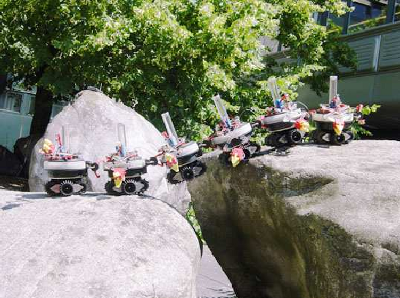
\includegraphics[width=10cm]{./img/sbot.png}
  \caption{Ukázka spolupráce robotů {\it s-bot}, kteří se snaží překonat překážku
    (propast), kterou jedinec sám překonat nedokáže.}
\end{figure}

Pro odlišení robotiky, která se zabývá hejny robotů, od ostatních směrů, které
studují multirobotické systémy, je třeba definovat, jakou oblast robotiky v sobě
zahrnuje {\it Swarm robotics}.

\begin{define} Oblast robotiky hejna se zabývá studiem
velkého počtu relativně jednoduchých, fyzicky realizovaných agentů, kteří jsou
navrženi tak, aby jejich požadované kolektivní chování bylo způsobeno pouze
lokálními interakcemi mezi agenty navzájem, případně mezi agenty a okolím.
\cite{Sahin05}
\end{define}

Na rozdíl od nerobotického swarmu, kde jedinec v roji či hejnu byl implementován
většinou na úrovni softwarové, je zde kladen důraz na fyzickou realizaci robota
a jeho umístění do reálného prostředí. Důležitou vlastností robotů v robotickém
hejnu je schopnost fyzicky interagovat s prostředím či ostatními roboty.

Shodnou vlastností hejn robotů některými uvedenými metodami (jako např. optimalizace
mravenčí kolonií) je decentralizovaná koordinace. Neexistuje zde žádný vůdce
nebo jedinec, který by direktivně řídil chování ostatních jedinců v hejnu.
Veškeré emergentní chování robotů tedy plyne pouze z lokální komunikace.

\subsubsection{Využití}
Protože je oblast robotiky hejna poměrně nová a zatím neexistují unifikované přístupy
pro návrh, implementaci a ladění robotických swarmů, není jejich komerční využití
příliš rozšířené. Mezi základní oblasti využití patří:
\begin{itemize}
  \item výrobní, provozní a inspekční systémy
  \item logistika, kooperativní transport
  \item vojenství (průzkum, robotický transport v neznámém prostředí)
  \item zemědělství
  \item medicína (mikrorobotika, kostní scintigrafie\cite{Rifaie11})
\end{itemize}


\subsection{Klasifikace a vlastnosti hejna robotů}
Hejno robotů můžeme klasifikovat podle různých úhlů pohledu na vlastnosti
či chování hejna \cite{Dudek93}:
\begin{itemize}
  \item {\bf Velikost hejna} {- počet robotů, kteří se pohybují v daném prostředí a tvoří hejno.}
  \item {\bf Komunikační dosah} {- ve většině systémů existují limity, které omezují
     možnosti komunikace robotů. Hlavním omezením je vzdálenost, na kterou mohou
     roboti komunikovat. Dalším faktorem může být schopnost adresace informace
     jinému robotovi, či všem robotům. Problémem může být také objem přenášených dat.}
  \item {\bf Rekonfigurace} {- míra schopnosti hejna změnit svoji topologii. Hejno může být buď
     statické (jedna topologie) a nebo dynamické, kde vztahy mezi jedinci se může měnit.}
  \item {\bf Výpočetní schopnost jedince} {- každý jedinec z hejna má určitou výpočetní schopnost
     odpovídající modelům, které jsou známé z teoretické informatiky. Můžeme tedy rozeznávat
     velmi jednoduché jedince, které pracují jako nelineární sumační jednotka - tyto jednotky
     pak mohou být využity pro výstavbu a simulaci neuronové sítě, ale obecně je tento model
     příliš jednoduchý, než aby se dali jedinci nazývat {\it roboty}. Dále lze uvažovat
     roboty, jejichž výpočetní model odpovídá konečnému automatu (což je preferovaným modelem
     u systémy se subsumpční architekturou). Další úrovní je zásobníkový automat, který není
     v robotice tak běžný a konečně Turingův stroj, což je výpočetní model používaný dnes
     většinou robotických systémů.}
\end{itemize}

\subsubsection{Vlastnosti systému}
Pokud se díváme na robotické hejno jako na systém, musí splňovat tyto vlastnosti,
které u jiných multirobotických systémů splněny většinou nejsou:
\begin{itemize}
  \item {\bf Robustnost} - robotický swarm by měl být schopen pracovat i za zhoršených
    podmínek okolí - např. při rušení či při selhání některých jedinců v hejnu. Hejna
    jsou typicky redundantním systémem - výpadek jednoho jedince může být velmi jednoduše
    a rychle nahrazen dalším. Aby bylo zamezeno častým selháním jedinců ve swarmu, měli by
    být poměrně jednoduché konstrukce na úrovni hardwarové i softwarové.
  \item {\bf Flexibilita} - hejno robotů by mělo být schopno řešit flexibilně různé úkoly.
    Inspirací v přírodě jsou mravenci, kteří díky komunikaci přes pachové stopy dokážou
    nalézt nejkratší cestu k potravě a současně jsou schopni společně velkou kořist odnést
    k mraveništi.
  \item {\bf Škálovatelnost} - použité koordinační mechanismy a strategie musí být schopny
    zajistit funkčnost swarmu při různých velikostech hejna.
  \item {\bf Homogenita} - jedinci ve swarmu by měli být homogenní, tj. buď by měli
    být identičtí z~hlediska architektury systému a schopnosti komunikace a interakce a
    nebo by měli splňovat alespoň požadavky na jednotné komunikační rozhraní a shodnost
    interakce s~okolními agenty a prostředím. Koordinační strategie, které jsou používány
    v~heterogenních multirobotických systémech, již nespadají pod přístup {\it swarm intelligence}.
\end{itemize}

\subsubsection{Požadavky na jedince}
Robotické swarmové systémy kladou na jedince (roboty) několik požadavků, které jsou
z hlediska robotiky pochopitelné, ale v oblasti obecné inteligence roje nejsou z důvodu
absence fyzické realizace zmiňovány. Těmito požadavky jsou:
\begin{itemize}
  \item {\bf Komunikace.} Propojení kabely a komunikace přes drátové připojení je jistě
    nedostatečné. Většina multirobotických a swarmových systémů by proto měla podporovat
    bezdrátovou komunikaci mezi roboty a také mezi konzolí a robotem pro snazší monitorování
    a ladění robotů. Dnes se v robotických systémech používají moduly založené na IR přenosu,
    dále IEEE 802.15.4/ZigBee (Kobot) a často také IEEE 802.11/Wi-Fi (s-bot, Centibot).
    Robot e-Puck je vybaven rozhraním pro komunikaci přes Bluetooth. V některých systémech
    (Kobot) bývají tyto kanály využívány také pro paralelní programování robotů ve swarmu.
  \item {\bf Fyzická interakce.} Roboti by měli umět fyzicky interagovat ve smyslu využití
    fyzických schopností svých i cizích pro dosažení určitého cíle (např. skládáním robotů
    do většího a silnějšího celku). Lze nahlédnout, že v některých aplikacích musí být robot
    dostatečně silný, aby dokázal druhého robota odtáhnout nebo aby jej dokázal nadzvednout.
  \item {\bf Výdrž.} Kvůli požadavku na vysokou flexibilitu robotů ve swarmu, by mělo být
    napájení realizováno pomocí výkonných baterií. Spotřeba robotů při plnění některých
    fyzických úloh může být poměrně vysoká, proto je třeba vzít tento fakt v úvahu.
  \item {\bf Velikost robota.} V některých systémech může být kladen důraz na velikost robota.
    Ta je vždy kompromisem; miniaturizace\ref{fig:jasmine} může být v některých případech velmi nákladná,
    naopak přílišné zmenšení systému je v protikladu s případnou rozšířitelností funkcionality
    robota.
  \item {\bf Simulovatelnost.} Vývoj robotického swarmu bez použití technik modelování
    a simulace by byl velmi obtížný, ne-li nemožný. Simulace by měla být zaměřena na
    model interakcí a komunikace mezi roboty a měla by realisticky popisovat fyzické
    schopnosti robotů.
\end{itemize}

\begin{figure}[here]
  \centering
  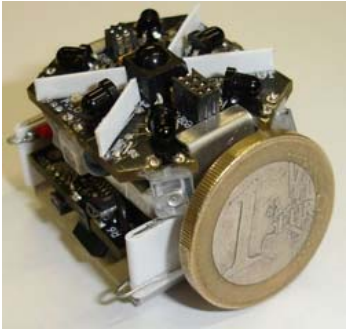
\includegraphics[width=7cm]{./img/jasmine.png}
  \caption{Miniaturizace robota pro swarm - na obrázku robot Jasmine s rozměry přibližně
    30x30x20mm. Zdroj: \url{http://www.swarmrobot.org/}}
  \label{fig:jasmine}
\end{figure}


\subsubsection{Koordinační mechanismy}
V přírodě nalezneme množství koordinačních mechanismů, které byly inspirací pro robotiku.
Uveďme tedy alespoň dva hlavní principy koordinace uvnitř swarmu.
\paragraph{Samoorganizace} {je v přírodních systémech běžná. Základním předpokladem pro
    výskyt jevů, které shrnujeme pod označení samoorganizace, je pozitivní a negativní
    odezva při lokální interakci jedinců \cite{Bonabeau99}. Dalším předpokladem je také
    existence náhody, která se v přírodě vyskytuje ve formě nepravidelností a mutací.}
\paragraph{Stigmergie} {je naopak mechanismem, který předpokládá nepřímou komunikaci
    mezi jedinci přes prostředí. Příkladem stigmergické komunikace je zanechávání feromonů
    na zemi; mravenci tímto způsobem označují cesty k potravě a tyto feromony pak působí
    jako atraktory.}

\subsubsection{Výpočetní schopnost robotického swarmu}
Robotické hejno se řadí do kategorie distribuované inteligence. Z pohledu teoretické
informatiky je jistě významné, se kterým výpočetním modelem je hejno robotů ekvivalentní.
Jistě záleží na výpočetních schopnostech jedince; avšak již u robotů, kteří jsou výpočetně
ekvivalentní konečnému automatu, lze dokázat ekvivalenci výpočetní schopnosti hejna těchto
robotů s Turingovým strojem.

Důkaz je založen na nekonečné množině komunikujících konečných automatů, u kterých jsou
rozlišeny tři druhy stavů: {\it vysílající, přijímající zleva a přijímající zprava}.
Základní myšlenkou pro simulaci Turingova stroje na této množině konečných automatů je
pak předpoklad, že každý automat simuluje konečné řízení Turingova stroje a reprezentuje
jedno pole na pásce. Automat korespondující s aktuálním polem na pásce je vždy ve stavu
{\it vysílající}, automat napravo je ve stavu {\it přijímající zleva} a automat
nalevo ve stavu {\it přijímající zprava}. Přechod vysílajícího automatu pak simuluje
posun čtecí hlavy doprava, doleva či přepis symbolu na pásce. Prostudování celého důkazu
pak v případě zájmu ponecháváme již na případném čtenáři. \cite{Dudek93}


\subsection{Typické problémy řešitelné hejny robotů}
Přestože komerční výroba systémů založených na robotice hejna není zatím příliš rozšířená
a výzkum probíhá spíše na akademických půdách a v laboratořích, jsou již známy úlohy,
které jsou pomocí těchto systémů řešitelné. Využitelnost robotického swarmu se pohybuje
v~oblastech, které jsou inspirovány přírodou. Tyto oblasti můžeme rozdělit na jisté {\it modely
chování}, jejichž zvládnutí pak představuje základ pro řešení složitějších úkolů a problémů.

\paragraph{Agregace} je obecný úkaz, kdy se jedinci seskupují do shluků, které mohou mít jistá
pravidla. Shlukování probíhá bez jakýchkoliv vodítek okolí a bez koordinace třetí stranou.
V robotice hejna se jedná o jeden z~nejdůležitějších modelů chování, ze kterého pak vychází
různé způsoby řešení problémů.
\paragraph{Disperze} (někdy označována jako segregace) je opakem agregace. Cílem u disperzního
swarmu je dosažení maximální plochy pokryté roboty tak, aby zůstávali stále ve spojení. Příkladem
takového chování jsou sami lidé, kteří tvoří "roje" když prohledávají hůře prostupný terén při
pátrání po nezvěstných nebo pohřešovaných osobách. Využitelnost robotického swarmu je nasnadě:
tuto práci by mohla převzít specializovaná hejna robotů, která by tyto osoby vyhledávala. Dalším
možným způsobem využití disperze je při předávání informací na velkou vzdálenost, kdy signál
od jednoho robota ke druhému nestačí (např. přenos informace na kilometry).
\paragraph{Vytváření vzorů} představuje obecný problém, který lze definovat jako vytváření
požadovaných geometrických obrazců a vzorů pomocí hejna robotů bez centralizované koordinace.
Toto chování není pouze geometrické, ale může být velmi funkční - v přírodě se vyskytuje například
ve formě vytvoření kruhovitého vzoru pro obklíčení kořisti skupinou predátorů.\\

Z těchto behaviorálních modelů\footnote{K těmto modelům lze ještě přiřadit pohyb propojených
robotů {\it (Connected Movement)}, který lze v některých případech považovat za jistý druh agregace.}
vychází problémy, které jsou řešitelné pomocí robotického swarmu \cite{Blum08SwarmInt}[96-97]:
\begin{itemize}
  \item {\bf Hledání zdrojů} {\it (Foraging)} lze zařadit do oblasti disperzního chování,
    což však není zcela přesné, protože většina přístupů pro vyhledávání (např. potravy)
    je založena na stigmergické komunikaci.
  \item {\bf Skládání} {\it (Self-assembly)} je úkaz pozorovaný u mravenců, kteří vytváření
    řetězcové formace, pomocí kterých vytváří "mosty", aby zůstali nad vodou. Problém skládání
    je nejčastěji řešen pomocí robotických chapadel nebo jiných mechanismů pro úchop a držení
    části dalšího robota. Skládání je typickým příkladem agregačního chování robotů.
  \item {\bf Kooperativní transport} {\it (Cooperative transport)} je jedním z nejzjevnějších
    druhů kooperativní inteligence pozorovaných u mravenců. Ti dokáží spojit své síly a
    transportovat tak k mraveništi kořist, která je mnohonásobně větší a těžší, než jeden
    mravenec. Principy kooperativního transportu spadají pod oblast agregačního chování hejna.
  \item {\bf Samoorganizovaná konstrukce} {\it (Self-organized construction)}, často označována
    také jako "agregace" byla jedním z~prvních problémů, které byly studovány v rámci inteligence
    hejna robotů. Jedná se o způsob chování, kdy roboti se snaží posbírat náhodně rozmístěné
    pasivní objekty na jedno místo.
\end{itemize}


\subsection{Návrh a modelování}
Cílem této kapitoly je představit základní koncepty a postupy při návrhu multirobotických
systémů, které vykazují emergentní chování plynoucí ze samoorganizace. Tyto metody lze
shrnout pod pojem "inženýrství samoorganizace" ({\it engineering of self-organization}).

Základním problémem při návrhu swarmových robotických systémů je určení konceptu
lokální komunikace mezi roboty tak, aby hejno vykazovalo požadované chování. Dalším
problémem je pak návrh vlastního fyzického zpracování robotů s ohledem na úkoly, které
mají společně plnit. V obecné rovině zatím neexistuje obecný postup či metodika pro návrh
takových systémů. Přístupy, které jsou dnes uplatňovány, by se daly rozdělit na dva
hlavní směry \cite[s.90-91]{Blum08SwarmInt}:

\paragraph{Ad-hoc přístup} je nejjednodušší metodou pro návrh swarmu. Návrhář se většinou
inspiruje chováním hmyzu v přírodě, abstrahuje z něj nejdůležitější znaky a parametry
a na jejich základě pak zformuluje algoritmus, jak dosáhnout požadovaného emergentního
chování u robotů. Přestože je tento přístup hojně využíván, skrývá v sobě nebezpečí v podobě
nízké úrovně laditelnosti a optimalizace celého procesu návrhu. I když je celková konstrukce
výsledného robota známa, může být problém nalézt optimální hodnoty pro všechny parametry systému.
Systematické experimentování pro nalezení těchto hodnot může být zdlouhavé a někdy i obtížně
realizovatelné.

\paragraph{Systémové přístupy} se nesnaží o návrh robotů, kteří pak dosahují očekávaného chování
v hejnu. Místo toho používají obecnou metodiku, která modeluje přímo požadované chování swarmu
a z modelu je pak odvozeno chování jedinců. Jedním z~těchto přístupů je umělá evoluce. Ve většině
studií (např. \cite{Dorigo05}) byla použita jednoduchá vícevrstvá dopředná nebo rekurentní neuronová síť,
která zakódovala chování hejna v simulovaném prostředí. Z tohoto modelu pak byly parametry
chování přeneseny do fyzického robota. Princip těchto přístupů je zobecněn na obrázku
\ref{fig:swarmdesign}.

\begin{figure}[here]
  \centering
  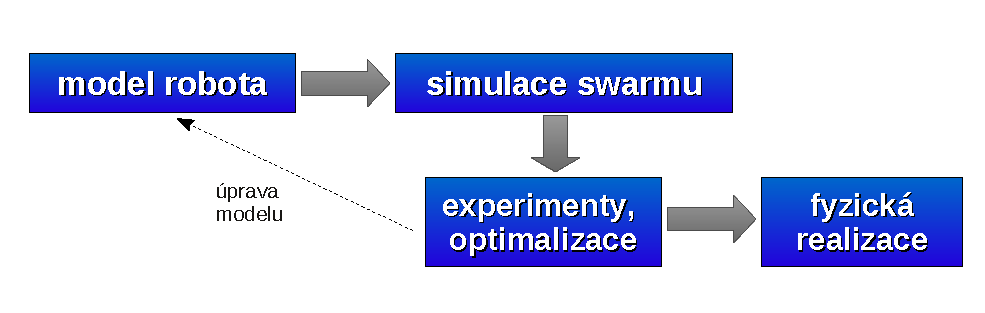
\includegraphics[width=14cm]{./img/swarm_rob_design.pdf}
  \caption{Princip návrhu robotického swarmu. Důraz je kladen na modelování a simulaci swarmu.}
  \label{fig:swarmdesign}
\end{figure}

\subsubsection{Modelování robotického hejna}
Jak již bylo zmíněno, modelování je často nedílnou součástí návrhu systémů založených na
hejnu robotů. Tyto systémy lze modelovat na různých úrovních abstrakce:
\begin{itemize}
  \item Modelování na úrovni senzorů
  \item Mikroskopické modelování
  \item Makroskopické modelování
\end{itemize}

\paragraph{Modelování na úrovni senzorů} je pravděpodobně nejpodrobnější z úrovní, na kterých
lze robotický systém smysluplně modelovat. Tento způsob je používán pro výstavbu realistických
simulátorů robotických systémů, ale pro modelování swarmu je třeba zajistit větší důraz na
úrovni komunikace a interakcí mezi roboty. Nevýhodou modelování na úrovni senzorů je vysoká
výpočetní náročnost simulace takových modelů. Simulace tak musí být paralelizovány a pro
výpočet bývají použity výkonné clustery počítačů.

\paragraph{Mikroskopické modelování} je podobné jako modelování na úrovni senzorů; model
je tvořen na úrovni jedince. Stavy robota a přechody mezi jeho stavy jsou modelovány analyticky.
Při použití této metody pak nejsou simulovány interakce jedinců uvnitř systému, ale model
je vystaven na vyšší úrovni. Tento přístup je co do modelování a simulace podstatně rychlejší,
než senzorově orientované modely a přitom poskytují dostatečně přesné parametry chování
a výstupy systému.

\paragraph{Makroskopické modelování} je na rozdíl od obou předchozích přístupů prováděno
na úrovni celého hejna. V modelu je zde reprezentován celkový stav systému a pro nalezení
stabilního stavu a optimálních hodnot parametrů je třeba model vyhodnotit pouze jednou.
Pokud by byl robotický systém modelován pomocí PFSM (pravděpodobnostní konečný automat),
v mikroskopickém modelování by každý robot odpovídal jednomu PFSM, zatímco při použití
makroskopického modelu by celé hejno bylo reprezentováno jedním PFSM\cite{Martinoli04}.



\subsection{Otázky}
\begin{enumerate}
  \item Čím se liší oblast {\it Swarm Robotics} (robotika hejn) od přístupů, které využívají
    inteligence roje pro optimalizaci?
  \item Jaké základní vlastnosti musí mít robotický systém, abychom jej klasifikovali jako swarm?
  \item Jaké požadavky klademe na roboty, které mají být využity v hejnu?
  \item Uveďte základní dva koordinační mechanismy, které se vyskytují uvnitř robotického hejna.
  \item Jaký je rozdíl mezi těmito modely chování robotů: agregace a disperze?
  \item Uveďte alespoň tři problémy, které jsou řešitelné pomocí hejna robotů.
  \item Popište principy uplatňované při návrhu robotického swarmu, proces ilustrujte na obrázku.
\end{enumerate}


\newpage
\renewcommand{\refname}{\section{Použitá literatura}}
\bibliographystyle{plain}
\bibliography{refs}

\end{document}
